\section{Evaluation}
\subsection{Research Questions}
To test our approach, we want to use our dataset of XWiki to answer the
following \acp{rq}:
\begin{itemize}
    \item \ac{rq}1: \emph{How many bug tickets are found when selecting only a subset of tests using NLP-Clustering by Test Specification}
          The goal of this paper is to demonstrate wether clustering tests in said method can produce helpful results. But is there actually a substantial amount of time/tests that can be saved when only selecting a portion of all tests?
    \item \ac{rq}2: \emph{How does the performance of NLP-based test selection compare with simpler, more naive methods of test selection in terms of bug detection and resource utilization?} This is done to show wether it is even worth it to implement something comparatively complex over something simple.
\end{itemize}

\subsection{Evaluation Metrics}
To evaluate how well our algorithm works, we want to find out how many bugs are
covered by a certain percentage of run tests. Our source also includes bug
tickets and we can link each test to its bug ticket. That way, we can go
through all n selected tests and make a set of bug tickets covered and divide
them by the number of all bug tickets and thereby know the percentage of bug
tickets covered. As we do not yet know how many tests should be selected, we
will go through all the percentage numbers from 10 to 70 in steps of ten and
see how many bug tickets have been covered by each number of tests.

\subsection{Comparison of Approaches}
To then find out how our algorithm compares to naive approaches we first have
to choose a naive approach. The first proposition that comes to mind is just
choosing n random tests from our test cases. Our alternative approach is only
possible with data that has some sort of categorization. As an example, the
test at
\begin{verbatim}
https://test.xwiki.org/xwiki/bin/view/File%20Manager%20Tests/Delete%20a%20file
\end{verbatim}
we mentioned earlier, is in the category \emph{P1.Extensions - File Manager
    Tests}. In total there are TODO categories like this in our data set. As we can
assume similar bugs belong to similar test categories, this implementation
might lead to a well enough grouping of test cases.

\subsection{Results}

We compared the three methods of test selection to evaluate their effectiveness
in covering bug tickets. These methods are represented in Table
\ref{table:bug_ticket_coverage_comparison} as:
\begin{itemize}
    \item Method 1, selecting test cases randomly from the entire dataset
    \item Method 2, selecting test cases randomly from each test category
    \item Method 3, being our presented approach with selecting tests by clustering test
          steps.
\end{itemize}

\begin{table}[H]
    \centering
    \renewcommand{\arraystretch}{1.5}  % Adjust the 1.5 to increase or decrease padding
    \begin{tabular}{|@{\hspace{5pt}}c@{\hspace{5pt}}|@{\hspace{5pt}}c@{\hspace{5pt}}|@{\hspace{5pt}}c@{\hspace{5pt}}|@{\hspace{5pt}}c@{\hspace{5pt}}|}  \hline
        Percentage of Tests Run & Method 1 & Method 2 & Method 3 \\ \hline
        10\%                    & 14.22\%  & 15.14\%  & 18.81\%  \\ \hline
        20\%                    & 26.15\%  & 27.75\%  & 36.24\%  \\ \hline
        30\%                    & 37.84\%  & 38.53\%  & 51.61\%  \\ \hline
        40\%                    & 47.25\%  & 47.94\%  & 59.86\%  \\ \hline
        50\%                    & 52.98\%  & 54.82\%  & 72.48\%  \\ \hline
        60\%                    & 69.95\%  & 68.35\%  & 80.96\%  \\ \hline
        70\%                    & 73.62\%  & 70.87\%  & 83.03\%  \\ \hline
    \end{tabular}
    \caption{Coverage of Bug Tickets by Percentage of Tests Run for Different Methods}
    \label{table:bug_ticket_coverage_comparison}
\end{table}

\begin{figure}[h]
    \centering
    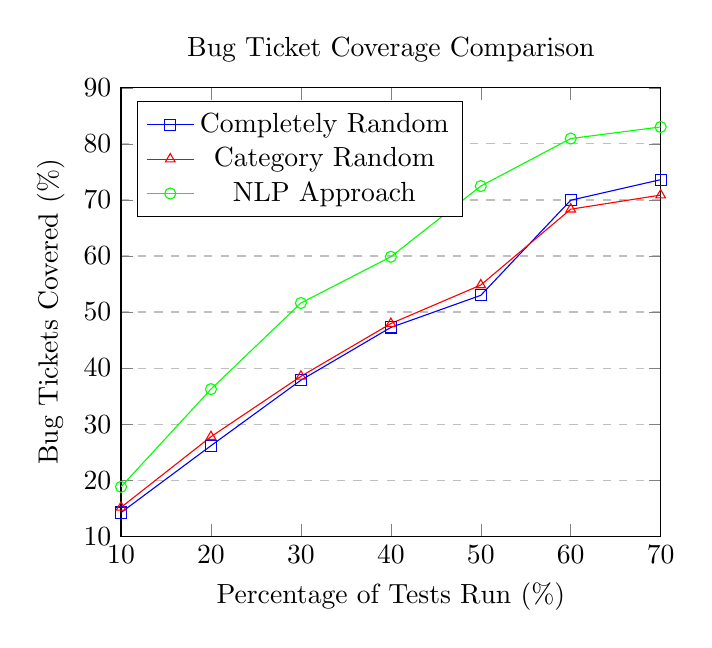
\begin{tikzpicture}
        \begin{axis}[
                title={Bug Ticket Coverage Comparison},
                xlabel={Percentage of Tests Run (\%)},
                ylabel={Bug Tickets Covered (\%)},
                xmin=10, xmax=70,
                ymin=10, ymax=90,
                xtick={10,20,30,40,50,60,70},
                ytick={10,20,30,40,50,60,70,80,90},
                legend pos=north west,
                ymajorgrids=true,
                grid style=dashed,
            ]

            \addplot[
                color=blue,
                mark=square,
            ]
            coordinates {
                    (10,14.22)(20,26.15)(30,37.84)(40,47.25)(50,52.98)(60,69.95)(70,73.62)
                };
            \addlegendentry{Completely Random}

            \addplot[
                color=red,
                mark=triangle,
            ]
            coordinates {
                    (10,15.14)(20,27.75)(30,38.53)(40,47.94)(50,54.82)(60,68.35)(70,70.87)
                };
            \addlegendentry{Category Random}

            \addplot[
                color=green,
                mark=o,
            ]
            coordinates {
                    (10,18.81)(20,36.24)(30,51.61)(40,59.86)(50,72.48)(60,80.96)(70,83.03)
                };
            \addlegendentry{NLP Approach}

        \end{axis}
    \end{tikzpicture}
    \caption{Comparison of different test selection approaches in terms of bug tickets covered.}
    \label{fig:bugticketcoverage}
\end{figure}

